\chapter{Расчет оптимальных стратегий выплаты дивидендов, перестрахования и инвестирования в диффузионной модели} \label{chapt:1}

\section{Постановка задачи} \label{sect:1.1}
Задача об оптимальной выплате дивидендов страховой компанией поставлена de Finetti \cite{DeF57}. Ее исследованию в различных постановках посвящено большое количество работ: см. обзоры \cite{Tak00, AlbTho09, Ava09}. Мы рассматриваем данную задачу в диффузионном приближении. В такой форме она впервые была поставлена в \cite{RadShe96, JeaShi95, AsmTak97}. Следует, однако, отметить, что математически эквивалентная задача исследовалась ранее в работе \cite{ShrLehGav84}.  В дальнейшем различные аспекты данной задачи были предметом многочисленных исследований. Большое внимание было уделено анализу оптимальных стратегий выплаты дивидендов при наличии возможностей стратегий перестрахования и инвестирования \cite{HogTak99, AsmHojTak00, HogTak04, CadChoTakZha06, MenSiu11, PelLae13}. В последнее время был проявлен значительный интерес к моделям с марковским переключениям параметров \cite{SotCad11, JiaPis12, ZhuChen13, Zhu14}, позволяющим учитывать влияние внешних случайных факторов.

В настоящей работе предполагается, что страховая компания может использовать стратегию перестрахования и инвестировать капитал в рисковый актив, динамика которого описывается моделью Блэка-Шоулза со случайным сносом. Целью работы является анализ влияния сноса, который колеблется около среднего значения и подчиняется процессу Орнштейна-Уленбека, на оптимальные стратегии выплаты дивидендов, перестрахования и инвестирования. Близкая модель с другим критерием оптимальности рассматривалась в \cite{LiaYueGuo11}.

Точная постановка задачи формулируется ниже в данном разделе. В разделе 2 устанавливается, что оптимальное значение задачи (функция Беллмана) является единственным вязкостным решением соответствующего уравнения Гамильтона-Якоби-Беллмана в полуплоскости. В разделе 3 рассматривается конечно-разностная аппроксимация данного уравнения и дается обоснование ее  сходимости. Заключительный раздел 4 посвящен обсуждению численных результатов.

Перейдем к постановке задачи. Следуя рассуждениям \cite{AsmHojTak00, HogTak04}, будем исходить из модели Крамера-Лундберга для резерва компании:
$$  R_t=x+pt-\sum_{i=1}^{N_t} Z_i.$$
Здесь $x$ --- начальный капитал, $p$ --- скорость поступления премий, $N_t(\lambda)$ --- пуассоновский процесс с постоянной интенсивностью $\lambda$, который описывает моменты поступления требований, и, наконец, $Z_i$ --- размер $i$-го требования. Предполагается, что случайные величины $Z_i$ неотрицательны, независимы, одинаково распределены, и имеют конечные математическое ожидание и дисперсию, и кроме того, $N_t$ и $Z_i$ независимы.

Пусть страховые премии вычисляются исходя из принципа среднего, тогда
$$ p t= (1+\eta)\mathsf E\left(\sum_{i=1}^{N_t} Z_i\right)=(1+\eta) t \lambda\mathsf E Z, $$
где $\eta>0$ --- коэффициент страховой нагрузки. Предположим теперь, что имеется возможность перестраховывать часть рисков, и обозначим через $Z^a$ величину ответственности страховой компании при поступлении требования размера $Z$. Типичными примерами являются пропроциональное перестрахование: $Z^a=a Z$, $a\in (0,1)$ или перестрахование эксцедента убытка: $Z^a=Z\wedge a$. Если скорость поступления премий $\widehat p$ перестраховщика вычисляется также на основе принципа среднего с коэффициентом нагрузки $\eta k(a)$, зависящим от $a$, то
$$ t\widehat p=(1+\eta k(a))\mathsf E\left(\sum_{i=1}^{N_t } (Z_i-Z_i^a)\right)=t(1+\eta k(a)) \lambda (\mathsf E Z-\mathsf E Z^a).$$
При этом резерв будет иметь вид
$$R_t=R_0+(p-\widehat p) t - \sum_{i=1}^{N_t } Z^a_i=x+(\lambda \mathsf E Z^a+\lambda\eta (\mathsf E Z-k(a)[\mathsf E Z-\mathsf E Z^a])t-\sum_{i=1}^{N_t} Z^a_i.$$

Одна из диффузионных аппроксимаций описана в работах \cite{AsmHojTak00, HogTak04}, где указано, что процесс $\eta R_{t/\eta^2}$ при $\eta\searrow 0$ слабо сходится к броуновскому движению с коэффициентами сноса и диффузии
$$ \mu_1(a)=\lambda (\mathsf E Z- k(a)[\mathsf E Z-\mathsf EZ^a]),\ \ \sigma_1^2(a)=\lambda\mathsf E\left[(Z^a)^2\right]$$
в пространстве $\mathbb D$ функций, непрерывных справа и имеющих пределы слева, наделенном топологией Скорохода. Таким образом, приходим к следующей модели резерва \cite{AsmHojTak00, HogTak04}:
\begin{equation} \label{eq:1.1.1}
d R_t=\mu_1(a) dt+\sigma_1 (a) dW^1_t,
\end{equation}
где $W^1$ --- стандартное броуновское движение.

Далее, пусть имеется рисковый актив, цена которого $S$ описывается стохастическим дифференциальным уравнением
\begin{equation} \label{eq:1.1.2}
dS_t= \mu_2 (Y_t) S_t dt +\sigma_2 (Y_t) S_t d W^2_t.
\end{equation}
Здесь $Y$ случайный фактор, динамика которого подчиняется уравнению
\begin{equation} \label{eq:1.1.3}
dY_t=\mu_3(Y_t)dt+\sigma_3 (Y_t) d W_t^3.
\end{equation}
Стандартные броуновские движения $(W^1,W^2,W^3)$ предполагаются независимыми. Модель, подобная (\ref{eq:1.1.2}), (\ref{eq:1.1.3}), рассматривалась в \cite{LiaYueGuo11}.

Предположим, что компания может инвестировать средства в данный актив, но объем этих инвестиций $\theta$ ограничен некоторой постоянной величиной $\overline\theta$. Пусть, кроме того, компания применяет динамическую стратегию $\alpha=(\alpha_t)_{t\ge 0}$ перестрахования и выплачивает дивиденды с конечной интенсивностью $c=(c_t)_{t\ge 0}$.
Приращение капитала $V$ компании складывается из приращений резерва, инвестированных средств и выплаченных дивидендов:
$$dV=dR+\theta\frac{dS}{S}- cdt.$$
Поставляя сюда выражения (\ref{eq:1.1.1}), (\ref{eq:1.1.2}), (\ref{eq:1.1.3}), находим
\begin{equation} \label{eq:1.1.4}
dV_t=(\mu_1(\alpha_t)+\mu_2(Y_t) \theta)dt +\sigma_1(\alpha_t) d W_t^1+\sigma_2(Y_t) \theta d W_t^2-c_t dt.
\end{equation}

Итак, фазовые переменные $(V,Y)$ --- капитал и внешний случайный фактор --- подчиняются системе (\ref{eq:1.1.3}), (\ref{eq:1.1.4}) стохастических дифференциальных уравнений. Пусть стратегия перестрахования $\alpha_t\in A$, стратегия инвестирования $\theta_t\in [0,\overline\theta]$ и интенсивность выплаты дивидендов $c_t\in [0,\overline c]$ прогрессивно измеримы относительно фильтрации, порожденной процессом $(W^1,W^2,W^3)$. Здесь $A$ --- компактное подмножество $\mathbb R$.

Полагая $X=(V,Y)^T$, $u=(\alpha,\theta,c)^T$, $W=(W^1,W^2,W^3)^T$, перепишем (\ref{eq:1.1.3}), (\ref{eq:1.1.4}) в более абстрактной форме
\begin{equation} \label{eq:1.1.5}
dX_t=b(X_t,u_t)dt+\sigma(X_t,u_t)dW_t,\quad X_0=x,
\end{equation}
$$ b=\begin{pmatrix}
  \mu_1(\alpha)+\mu_2(Y) \theta-c \\
  \mu_3(Y)
 \end{pmatrix},\ \ \
\sigma=\begin{pmatrix}
  \sigma_1(\alpha) & \sigma_2(Y) \theta & 0\\
   0 & 0 & \sigma_3 (Y)
	\end{pmatrix}.
$$
Для существования сильного решения системы (\ref{eq:1.1.5}) на интервале $[0,\infty)$ наложим на ее коэффициенты стандартные условия Липшица и линейного роста \cite[гл.\,2, \S 5]{Kry77}. Как легко видеть, для этого достаточно, чтобы функции $\mu_2, \sigma_2, \mu_3, \sigma_3$ были непрерывны по Липшицу:
$$ |\mu_i(y_1)-\mu_i(y_2)|+|\sigma_i(y_1)-\sigma_i(y_2)|\le K|y_1-y_2|,\ \ i=2,3$$
с константой $K$, не зависящей от $y_1$, $y_2$.

Обозначим через $X^{x,u}$ решение системы (\ref{eq:1.1.5}) при заданной стратегии управления $u=(\alpha,\theta,c)$. Цель компании состоит в максимизации ожидаемой дисконтированной суммы выплаченных дивидендов до момента банкротства:
\begin{equation} \label{eq:1.1.6}
v(x)=\sup_{u}\mathsf E \int\limits_{0}^{\tau^{x,u}} e^{-\beta t} c_t dt.
\end{equation}
Здесь $\tau^{x,u}=\inf\{t\ge 0: X_t^{x,u}\le 0\}$, $\beta>0$ и максимизация ведется по всем прогрессивно измеримым управлениям
$$ u_t=(\alpha_t,\theta_t,c_t)\in U:=A\times [0,\overline\theta]\times [0,\overline c].$$

%\newpage
%============================================================================================================================
\section{Уравнение Гамильтона-Якоби-Беллмана} \label{sect:1.2}
Из теории стохастического оптимального управления (см. \cite{Kry77, Pha09, Tou13}) известно, что, по крайней мере формально, функция Беллмана $v$ в полуплоскости $G=(0,\infty)\times \mathbb R$ удовлетворяет уравнению Гамильтона-Якоби-Беллмана
\begin{equation} \label{eq:1.2.1}
\beta v(x) - H(x,v_x(x),v_{xx}(x))=0,\ \  x\in G
\end{equation}
с гамильтонианом
$$ H(x,p,M)=\sup_{(a,c)\in U} \left[c+b(x,a,c)\cdot p + \frac{1}{2}\Tr(\sigma(x,a,c)\sigma^T(x,a,c)M))\right],$$
$p\in\mathbb R^d$, $M\in\mathbb S^d$. Мы используем обозначения $v_x=(v_{x_i})_{i=1}^n$, $v_{xx}=(v_{x_i x_j})_{i,j=1}^n$ для градиента и гессиана, и $\mathbb S^d$ --- для множества $d\times d$ симметрических матриц. На границе полуплоскости должно выполняться условие Дирихле:
\begin{equation} \label{eq:1.2.2}
v(x)=0,\ \ x\in\partial G.
\end{equation}

Задачу (\ref{eq:1.2.1}), (\ref{eq:1.2.2}) можно переписать также в виде
\begin{align} \label{eq:1.2.1A}
 \beta v(x) &-\mu_3(x_2) v_{x_2}(x)-\frac{1}{2}\sigma_3^2(x_2) v_{x_2 x_2}-\max_{\theta\in [0,\overline\theta]}\{\mu_2(x_2)\theta v_{x_1}(x)+\frac{1}{2}\sigma_2^2(x_2)\theta^2 v_{x_1 x_1}\}\nonumber\\
&- \max_{c\in [0,\overline c]}\{(1-v_{x_1}(x))c\}-\sup_{a\in A}\{\mu_1(a)v_{x_1}(x)+\frac{1}{2}\sigma_1^2(a)v_{x_1 x_1}(x)\}=0,\\
v(0,x_2) &=0.\nonumber
\end{align}

Более точно, данную краевую задачу следует понимать в <<вязкостном смысле>>. Напомним соответствующие определения \cite{CraIshLio92, Pha09, Tou13, Jak10}. Введем функцию $F:\overline G\times\mathbb R\times\mathbb R^d\times\mathbb S^d\mapsto\mathbb R$ по формуле
$$ F(x,r,p,M)=\left\{\begin{array}{l l}
    \beta r-H(x,p,M), & x\in G,\\
    r, & x\in\partial G.
  \end{array} \right.$$
Пусть $F_*$, $F^*$ полунепрерывная снизу и полунепрерывная сверху оболочки $F$.
Ограниченная полунепрерывная сверху (соотв., снизу) функция $u$ называется \emph{вязкостным субрешением} (соотв., \emph{вязкостным суперрешением}) задачи (\ref{eq:1.2.1}), (\ref{eq:1.2.2}), если для любой функции $\varphi\in C^2(\overline G)$ и любой точки $x_0\in\overline G$ локального максимума (соотв., локального минимума) функции $u-\varphi$ на $\overline G$ выполняется неравенство
$$ F_*(x_0,u(x_0),\varphi_x(x_0),\varphi_{xx}(x_0)) \le 0,$$
$$ \left(\text{соотв.,}\ \ F^*(x_0,u(x_0),\varphi_x(x_0),\varphi_{xx}(x_0)) \ge 0\right). $$

Такая форма записи позволяет не разделять уравнение и граничное условие. В частности, условие, определяющее субрешение, может быть переписано следующим образом:
\begin{align*}
\beta u(x_0) - H(x_0,\varphi_x(x_0),\varphi_{xx}(x_0)) & \le 0,\ \ x_0\in G,\\
\min\{\beta u(x_0) - H(x_0,\varphi_x(x_0),\varphi_{xx}(x_0)),u(x_0))\} & \le 0,\ \
x_0\in\partial G.
\end{align*}

Ограниченная функция $u$ называется \emph{вязкостным решением} задачи (\ref{eq:1.2.1}), (\ref{eq:1.2.2}) если ее полунепрерывная сверху и полунепрерывная снизу оболочки (по отношению к $\overline G$) являются соответственно вязкостными суб- и суперрешениями.

Хорошо известно (см. \cite[следствие 5.11]{Jen89}, \cite[раздел 1.1]{BarBot98}), что если область $G$ ограничена, то из свойства непрерывности по Липшицу коэффициентов уравнения и компактности множества $U$ вытекает, что для любых субрешения $u$ и суперрешения $v$ уравнения (\ref{eq:1.2.1}) (т.е., формально говоря, задачи (\ref{eq:1.2.1}), (\ref{eq:1.2.2}) в области $G$), удовлетворяющих условию $u\le w$ на $\partial G$, имеет место неравенство $u\le w$ на $G$. При этом говорят, что справедлив \emph{принцип сравнения}. Отправным пунктом доказательства является так называемое \emph{структурное условие}, которому удовлетворяет $F$ (см. также \cite{CraIshLio92}, \cite[предположение 6.20]{Tou13}). Случай неограниченной области рассмотрен в \cite[теорема 7.3]{Ish89}, \cite[теорема 6.21]{Tou13}.

Обозначим через $\mathcal U^-$ (соотв., $\mathcal U^+$) множество вязкостных субрешений $u$ (соотв., вязкостных суперрешений  $w$) уравнения (\ref{eq:1.2.1}), для которых $u\le 0$ (соотв., $w\ge 0$) на $\partial G$. Заметим, что множества $\mathcal U^-$, $\mathcal U^+$ непусты: $0\in\mathcal U^-$, $\overline{c}/\beta\in\mathcal U^+$.
Из принципа сравнения вытекает, что выполняется неравенство
\begin{equation} \label{eq:1.2.3}
\underline h(x):=\sup_{u\in\mathcal U^-} u(x)\le\overline h(x):=\inf_{w\in\mathcal U^+} w(x),\ \ x\in\overline G.
\end{equation}
Согласно \cite{BarBot98} функция $\underline h$ (соотв., $\overline h$) называется \emph{нижним} (соотв., \emph{верхним}) $e$-\emph{решением} задачи (\ref{eq:1.2.1}), (\ref{eq:1.2.2}). Если неравенство (\ref{eq:1.2.3}) является равенством, то функция $h=\underline h=\overline h$ называется $e$-решением. Из наличия субрешения $u=0$, удовлетворяющего граничному условию (\ref{eq:1.2.2}), вытекает (см. \cite[теорема 2]{BarBot98}), что $e$-решение существует и совпадает с наименьшим верхним $e$-решением, т.е. $h\in\mathcal U^+$.

Поставленная задача (\ref{eq:1.1.6}) может быть включена в класс задач о максимизации времени выхода вырожденного диффузионного процесса из области, который рассмотрен в \cite{BarBot98} (раздел 3.2). Заметим, что сделанное в указанной работе дополнительное предположение об ограниченности коэффициентов $b$, $\sigma$ несущественно. В теореме 9 работы \cite{BarBot98} установлено, что функция Беллмана $v$, определенная формулой (\ref{eq:1.1.6}), совпадает с $e$-решением задачи (\ref{eq:1.2.1}), (\ref{eq:1.2.2}): $v=h$ на $\overline G$. В частности, отсюда следует, что $v$ полунепрерывна снизу.

Предположим теперь, что в нашей задаче выполняется следующее условие невырожденности
\begin{equation} \label{eq:1.2.4}
\underline{\sigma}_1:=\inf_{a\in A}\sigma^1(a)>0.
\end{equation}
В этом случае справедлив \emph{сильный принцип сравнения}: для любых субрешения $u$ и суперрешения $v$ задачи (\ref{eq:1.2.1}), (\ref{eq:1.2.2}) имеет место неравенство $u\le w$ на $G$. Данный результат является следствием невырожденности диффузии по нормали к границе (см. \cite{BarBur95, BarRou98}), что в данном означает (\ref{eq:1.2.4}). Его доказательство сводится к обычному принципу сравнения, так как из условия (\ref{eq:1.2.4}) вытекает, что любые вязкостные субрешение $u$ и суперрешение $w$ задачи (\ref{eq:1.2.1}), (\ref{eq:1.2.2}) удовлетворяют граничным условиям в обычном смысле: $u\le 0$, $v\ge 0$ на $\partial G$ (см. предложение 1.1 работы  \cite{BarBur95} и его доказательство).

Наконец, из сильного принципа сравнения вытекает, что функция Беллмана $v$ непрерывна и является единственным вязкостным решением задачи (\ref{eq:1.2.1}), (\ref{eq:1.2.2}): см. \cite{Rok14} (теорема 1 и замечание 1).


Заметим, что если условие (\ref{eq:1.2.4}) не выполняется, то для вычисления $v$ могут быть использованы различные схемы аппроксимации: см. \cite{BarBot98} (раздел 2).

\section{Разностная схема} \label{sect:1.3}
Для численного решения задачи рассмотрим прямоугольную сетку
$$\overline G_h=\{(ih_1,jh_2):0\le i\le I,-J\le j\le J\},\ \ \  Ih_1=a,\ \ Jh_2=b.$$
Здесь $I,J,i,j$ --- целые числа, $h=(h_1,h_2)$ --- шаг сетки. Узлы $(ih_1,jh_2)$, $0<i<I$, $-J<j<J $ назовем внутренними, а остальные узлы --- граничными. Множества внутренних и граничных узлов обозначим через $G_h$ и $\partial G_h$ соответственно. Каждому внутреннему узлу поставим в соответствие уравнение для сеточной функции $v_{ij}=v(x_{ij})$, $x_{ij}=(ih_1,jh_2)$:
\begin{align*}
0 &=\beta v_{ij} -\left(\mu_{3;j}^+ \frac{v_{i,j+1}-v_{ij}}{h_2}-\mu_{3;j}^-\frac{v_{i,j}-v_{i,j-1}}{h_2}\right)-\frac{1}{2}\sigma_{3;j}^2 \frac{v_{i,j+1}-2 v_{ij}+v_{i,j-1}}{h_2^2}  \\
&-\max_{\theta\in [0,\overline\theta]}\left\{\mu_{2;j}^+\theta \frac{v_{i+1,j}-v_{ij}}{h_1} -\mu_{2;j}^- \theta \frac{v_{i-1,j}-v_{i,j}}{h_1} +\frac{1}{2}\sigma_{2;j}^2\theta^2 \frac{v_{i+1,j}-2 v_{ij}+v_{i-1,j}}{h_1^2}\right\}\\
&-\max_{c\in [0,\overline c]} \left\{c\left(1-\frac{v_{ij}-v_{i-1,j}}{h_1}\right)\right\}\\
& -\max_{a\in A}\left\{\mu_1^+(a) \frac{v_{i+1,j}-v_{i,j}}{h_1}-\mu_1^-(a) \frac{v_{ij}-v_{i-1,j}}{h_1}+\frac{1}{2}\sigma_1^2(a)\frac{v_{i+1,j}-2 v_{ij}+v_{i-1,j}}{h_1^2}\right\}.
\end{align*}
Здесь $\mu_{k;j}=\mu_k(jh_2)$, $\sigma_{k;j}=\sigma_k(jh_2)$, $k=2,3$. В граничных узлах  ставится условие Дирихле
$$ 0=v_{ij},\ \ i\in\{0,I\},\ j\in \{-J,\dots,J\};\ \ i\in [0,\dots,I],\ \ j\in\{-J,J\}.$$
Данную систему уравнений представим в виде
\begin{equation} \label{eq:1.3.1}
0=F_h(x_{ij},v_{ij},(v_{ij}-v_{i'j'})_{x_{i'j'}\in\Gamma(x_{ij})}),\ \ x_{ij}\in \overline G_h,
\end{equation}
где $\Gamma(x_{ij})$ --- множество узлов, соседних с $x_{ij}$:
$$\Gamma(x_{ij})=\{x_{i+1,j},x_{i-1,j},x_{i,j+1},x_{i,j-1}\}\ \ \text{для }\ x_{ij}\in G_h$$
и $\Gamma(x_{ij})=\varnothing$ для $x_{ij}\in \partial G_h$.

Выбранный способ аппроксимации первых производных обеспечивает неубывание функций $F_h$ по всем аргументам, за исключением $x_{ij}$. В терминологии \cite{Obe06} это означает, что схема является \emph{вырожденной эллиптической}. Кроме того, выполняется неравенство
$$ F_h(x,r,y)-F_h(x,r',y)=\beta' (r-r')>0, \ \ \beta'=\min\{\beta,1\}\ \ \text{при}\ r>r',$$
означающее, что схема является \emph{правильной} (\emph{proper}) \cite{Obe06}. Далее, построенная схема является \emph{непрерывной по Липшицу} с константой $K_h$:
$$ | F_h(x,z)-F_h(x,z')|\le K_h \|z-z'\|_{\infty}.$$
Здесь $\|z\|_\infty=\max\{|z_{ij}|:z_{ij}\in \overline G_h\}$.

Простые оценки, основанные на элементарном неравенстве
\begin{equation} \label{eq:1.3.2}
|\max_{q\in Q}\psi(x,q)-\max_{q\in Q}\psi(y,q)|\le\max_{q\in Q} |\psi(x,q)-\psi(y,q)|,
\end{equation}
справедливом для непрерывной функции $\psi$ и компактного множества $Q$, показывают, что константа $K_h$ может быть определена следующим образом:
\begin{align*}
K_h=\beta &+ \frac{\|\mu_3\|_\infty}{h_2}+\frac{\|\sigma_3^2\|_\infty}{h_2^2}+
\frac{\overline\theta\|\mu_2\|_\infty+\overline c+\sup_{a\in A}|\mu_1(a)|}{h_1}\\
 &+ \frac{\overline\theta^2 \|\sigma_2^2\|_\infty+\sup_{a\in A}|\sigma_1^2(a)|}{h_1^2}.
\end{align*}

В работе \cite{Obe06} (теорема 7) показано, что оператор $S_\rho(v)=v-\rho F_h[v]$,
действующий в пространстве сеточных функций с нормой $\|\cdot\|_\infty$, является строгим сжатием при достаточно малых $\rho$:
$$ \| S_\rho(u)-S_\rho(v)\|_\infty\le\gamma\|u-v\|_\infty,\ \ \gamma=\max\{1-\rho\beta',\rho K_h\}.$$
Отсюда следует, что система уравнений (\ref{eq:1.3.1}) имеет единственное решение $v_h$, совпадающее с неподвижной точкой $S_\rho$, и оно может быть найдено  методом простых итераций:
\begin{equation}  \label{eq:1.3.3}
 v^{n+1}=S_\rho(v^n),\ \ \|v_h-v^n\|_\infty\to 0
\end{equation}
с произвольным начальным приближением $v^0$.

Для обоснования сходимости сеточных функций $v_h$, $h\to 0$ к функции Беллмана $v$ воспользуемся методом \cite{BarSou91}.

Как было отмечено выше, в предположении (\ref{eq:1.2.4}) неравенство $u(x)\le w(x)$, $x\in\overline G$ выполняется для любых вязкостных суб- и суперрешений $u$ и $w$ задачи (\ref{eq:1.2.1}), (\ref{eq:1.2.2}). Таким образом, в терминологии \cite{BarSou91}, выполняется свойство \emph{сильной единственности}. Но тогда локально равномерная сходимость $v_h$ к $v$ является следствием свойств устойчивости, монотонности и согласованности разностной схемы: \cite[теорема 2.1]{BarSou91}. Рассмотрим данные свойства более подробно.

Для вырожденных эллиптических правильных схем из неравенства $F_h[u_h]\le F_h[w_h]$ вытекает, что $u_h\le w_h$ \cite[теорема 5]{Obe06}. Поскольку
$$ F_h[0]\le F_h[v_h]=0\le F_h[\overline{c}/\beta],$$
то отсюда вытекают неравенства $0\le v_h\le\overline{c}/\beta$, означающие, что выполняется условие \emph{устойчивости} \cite{BarSou91}:
$$\sup_h\|v_h\|_\infty\le \overline{c}/\beta.$$
Условие \emph{монотонности} \cite{BarSou91} сводится к условию невозрастания функций
 $$F_h(x_{ij},v_{ij},(v_{ij}-v_{i'j'})_{i'j'\in N(i,j)})$$
по переменным $v_{i'j'}$, что вытекает из вырожденной эллиптичности схемы.

Возьмем последовательность сгущающихся сеток на расширяющейся системе прямоугольников, т.е. будем считать, что $I=I_{h^n}$, $J=J_{h^n}$ зависят от $h^n=(h_1^n,h_2^n)\to 0$ таким образом, что $a^n=I_{h^n} h_1^n\to\infty$, $b^n=J_{h^n} h_2^n\to\infty$. Пусть, кроме того, для любой точки замкнутой полуплоскости $x\in\overline G$ существует последовательность $x_{i_n j_n}\in\overline G_{h_n}$: $x_{i_n j_n}\to x$.

Чтобы установить \emph{согласованность} схемы по \cite{BarSou91} нужно доказать, что для любых бесконечно гладкой равномерно ограниченной функции $\varphi\in C_b^\infty(\overline G)$ и последовательности $\xi_n\searrow 0$ справедливы неравенства
\begin{equation} \label{eq:1.3.4}
\liminf_{n\to\infty} F\left(x_{i_n j_n},\varphi(x_{i_n j_n})+\xi_n,(\varphi(x_{i_n j_n})-\varphi(y))_{y\in\Gamma(x_{i_n j_n})}\right)\ge
F_*(x,\varphi(x),\varphi_x(x),\varphi_{xx}(x)),
\end{equation}
\begin{equation} \label{eq:1.3.5}
\limsup_{n\to\infty} F\left(x_{i_n j_n},\varphi(x_{i_n j_n})+\xi_n,(\varphi(x_{i_n j_n})-\varphi(y))_{y\in\Gamma(x_{i_n j_n})}\right)\le
F^*(x,\varphi(x),\varphi_x(x),\varphi_{xx}(x)).
\end{equation}
Обозначения $F_*$, $F^*$ введены в разделе 2.

Простые, но громоздкие вычисления, основанные на формуле Тейлора и неравенстве (\ref{eq:1.3.2}), позволяют установить, что
\begin{equation} \label{eq:3.6}
\lim_{n\to\infty} F\left(x_{i_n j_n},\varphi(x_{i_n j_n})+\xi_n,(\varphi(x_{i_n j_n})-\varphi(y))_{y\in\Gamma(x_{i_n j_n})}\right)=F(x,\varphi(x),\varphi_x(x),\varphi_{xx}(x)),
\end{equation}
если последовательность $(x_{i_n j_n})$ состоит из внутренних точек полуплоскости $\overline G$. Если же данная последовательность состоит из граничных точек, то равенство (\ref{eq:3.6}) выполняется тривиальным образом. Отсюда легко следуют неравенства (\ref{eq:1.3.4}), (\ref{eq:1.3.5}).

\section{Результаты численных расчетов} \label{sect:1.4}
При проведении численных экспериментов рассматривался частный случай исследуемой модели, в которой волатильность $\sigma_2$ рискового актива $S$ постоянна, а снос $\mu_2$ подчиняется процессу Орнштейна-Уленбека:
%\begin{align*}
$$\mu_2(Y)  =l+ k_1 Y,\quad  dY=-k_2 Y dt + \sigma_3 dW^3. $$
Здесь $l$, $k_1$, $k_2$, $\sigma_3$ --- положительные константы. Как отмечено, напр.,  в \cite{Ris99, LiaYueGuo11} такая модель позволяет описывать черты, присущие рынкам <<быков>> и <<медведей>>.

Кроме того, рассматривался пропорциональный механизм перестрахования рисков в случае дешевого перестрахования (cheap reinsurance) \cite{AsmHojTak00}: $Z^a=aZ$, $k(a)=1$. При этом, в предположении $\lambda=1$,
\begin{equation}
\mu_1(a)=a \overline\mu,\quad \sigma_1 (a)=a\overline\sigma,
\end{equation}
где  $\overline\mu=\mathsf E Z$, $\overline\sigma^2=\mathsf E Z^2$.

Численные эксперименты проводились при следующих значениях параметров:  $l=0.05$, $k_1=0.05$, $\sigma_2=0.4$, $\sigma_3=0.5$, $\overline\mu  =0.2$, $\overline\sigma=0.5$, $\overline c=5$, $\overline\theta=20$, $\beta=0.05$. В качестве множества $A$ допустимых уровней перестрахования $\alpha$ был выбран интервал $[\varepsilon,1]$, $\varepsilon=10^{-6}$. Для анализа влияния на оптимальное решение скорости возврата процесса $Y$ к равновесному значению $0$ рассматривались значения параметра $k_2=0.1 , 1, 10$. Кроме того, рассматривался случай $\mu_3=0$, $\sigma_3=0$, что соответствует одномерной модели с фиксированным уровнем внешнего случайного фактора $Y_t = Y_0=x_2$.

Расчеты проводились в прямоугольнике $[0,\overline x_1]\times [\underline x_2,\overline x_2]$, $\overline x_1=9$, $\underline x_2=-5$, $\overline x_2=20$  на сетке с шагами $h_1=0.05$, $h_2=0,042$. Таким образом, сетка состояла из $180*600$ узлов с учетом граничных. Параметр $\rho$ в методе простых итераций $(\ref{eq:1.3.3})$ определялся по формуле $\rho=1/(2 K_h)$. В качестве начальных приближений выбирались $\underline v^0=0$ и $\overline v^0= \overline c / \beta$, которые являются грубыми оценками оптимального значения решения $v_h$ задачи (\ref{eq:1.3.1}) снизу и сверху соответственно.  Заметим, что из монотонности схемы (\cite[теорема 6]{Obe06}) вытекает, что неравенство $\underline v^n\le\overline v^n$ между соответствующими приближениями сохраняется при всех $n$.

Алгоритм отрабатывал число итераций необходимое, чтобы максимальная относительная погрешность
$$ \max_{ij}\frac{|\underline v^n_{ij}-\overline v^n_{ij}|}{\underline v^n_{ij}}$$
между между приближениями не превышала  2\%.
При рассматриваемых параметрах для одномерной задачи с параметром $x_2$ для этого требуется это около $4.5$ миллионов итераций, а для двумерного --- от 6 до 8 миллионов итераций в зависимости от значения параметра $k_2$.

Для программирования использовался язык <<Си>>. Расчеты проводились на процессоре <<Intel Core i5-3230M>> с тактовой частотой $2.6$ Ггц. При обычном запуске программы на один эксперимент затрачивалось от $11$ до $20$ часов. Однако, так как данный процессор может одновременно работать с четырьмя потоками, то, используя технику параллельного программирования, удалось ускорить работу алгоритма примерно в $3.8$ раза. При этом на самый длительный эксперимент затрачивалось чуть более $5$ часов.

На представленных ниже рисунках сплошная линия, отмеченная цифрой 1, соответствует одномерной задаче $(\mu_3=\sigma_3=0)$  с параметром $Y_t=x_2$. Цифры 2, 3, 4 и соответствующие им линии относятся к значениям параметра $k_2=0.1 , 1, 10$.

Из представленных на рис.\,\ref{fig:1.1} графиков, видно что функция Беллмана $v$ является возрастающей и вогнутой по $x_1$. Типичная картина, состоит в том, что при малых $x_2$ функция Беллмана двумерной задаче мажорирует функцию Беллмана одномерной задачи, а при больших $x_2$ --- наоборот. Переходная область определяется уровнем $\mu_2=l$, а данные свойства --- <<притягиванием>> $Y$ к нулевому уровню в двухмерной задаче. Например, если $x_2<0$, то в одномерной задаче эта ситуация не изменится, а в двумерной снос $\mu_2$ увеличится, что создает более благоприятную ситуацию для инвестирования.

\begin{figure}[h]
        \centering
          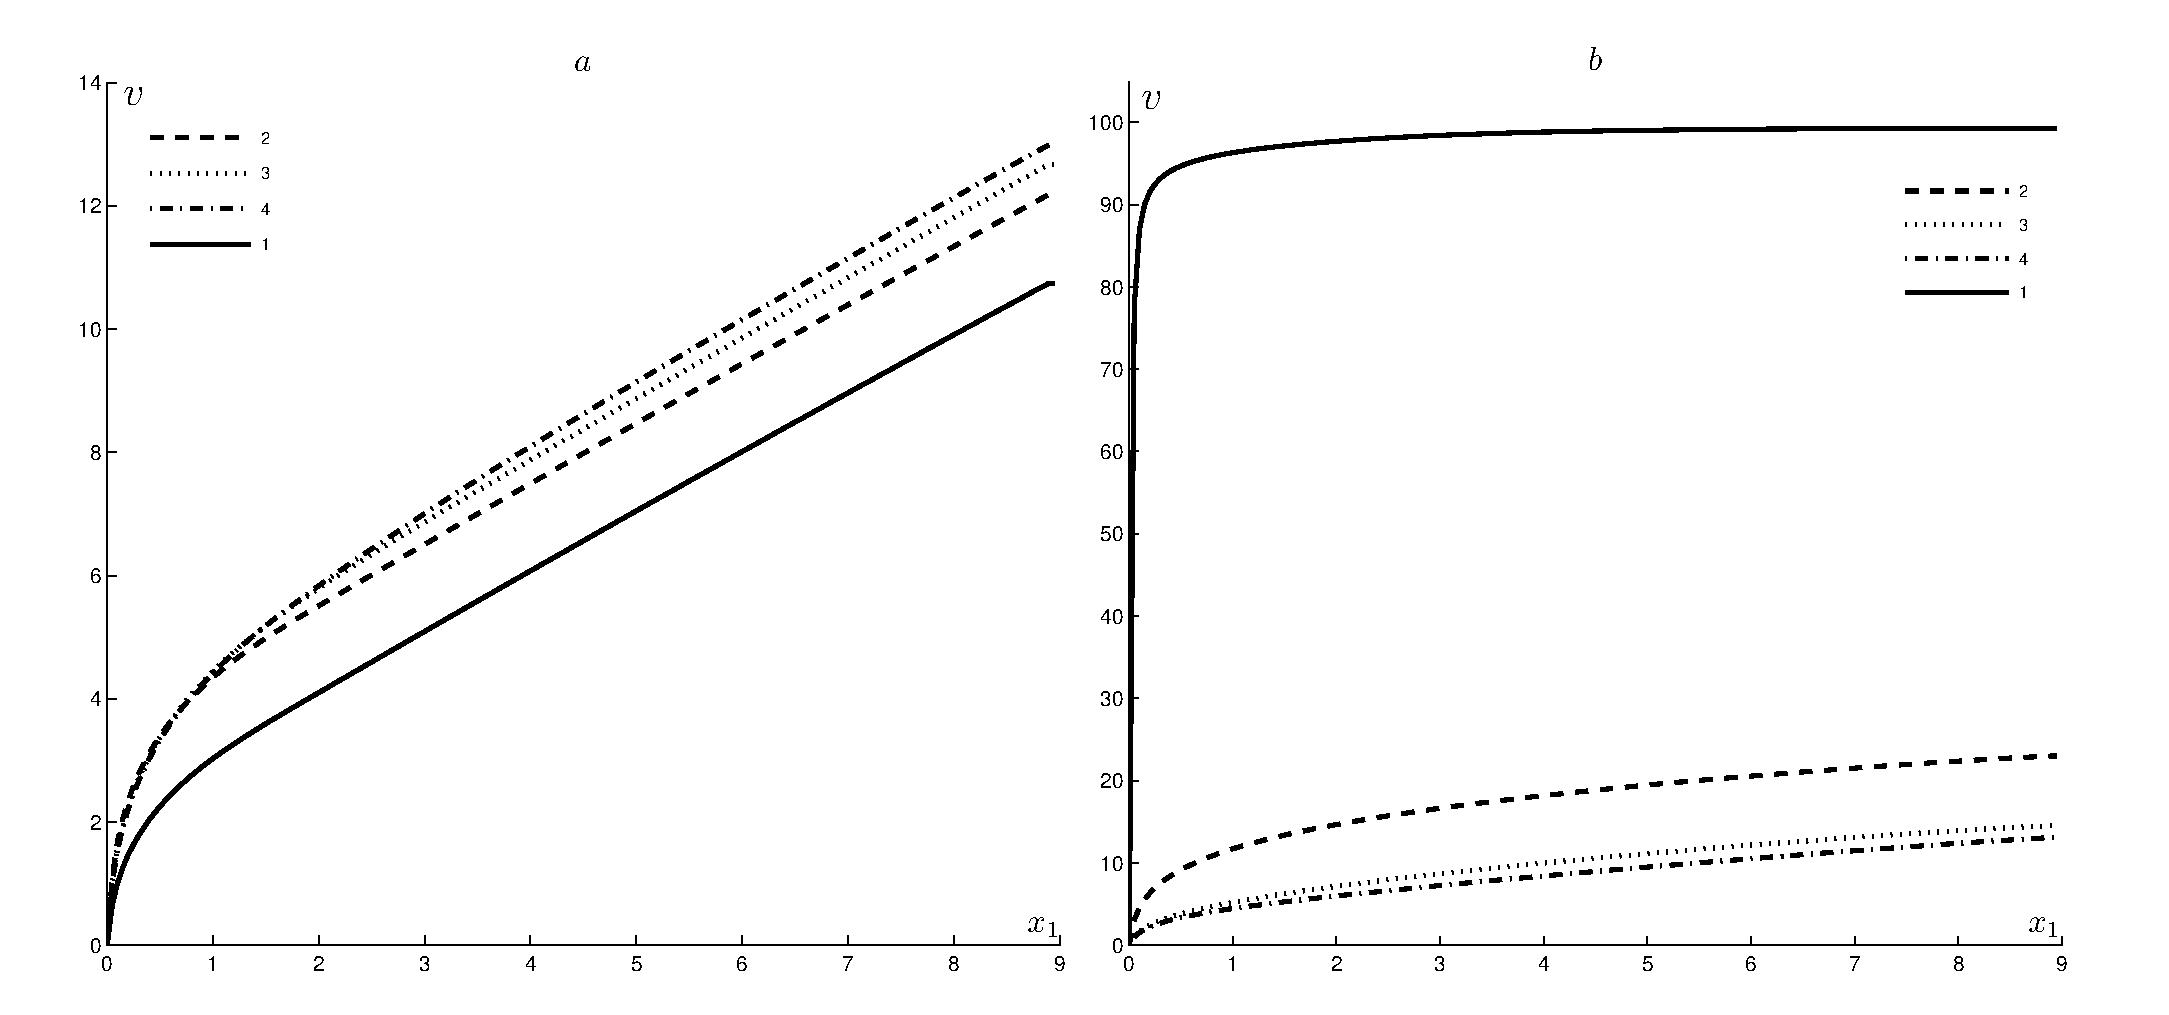
\includegraphics[width=0.9\textwidth]{V_y.eps}
         \caption{Графики сечений функции Беллмана $v(\cdot,x_2)$, (a) $x_2=-1.88$, (b) $x_2=4.58$.}
          \label{fig:1.1}
\end{figure}

Не приводя соответствующих графиков, отметим, что по переменной $x_2$ наблюдается монотонный рост функции $v$ и ярко выраженная выпуклость в одномерном случае. Сверхлинейный рост $v$ по $x_2$ можно объяснить тем, что вместе с $x_2$ растет оптимальное значение $\theta^*$.

Перейдем к рассмотрению оптимальных стратегий. Численные расчеты подтверждают хорошо известную <<барьерную>> структуру оптимальной интенсивности $c^*$ выплачиваемых дивидендов:
\begin{equation}
 \begin{matrix}
c^* & = & \left \{
\begin{matrix} 0,& x_1< x^*(x_2) \\
               \overline c,& x_1 \ge x^*(x_2).
\end{matrix}\right.
\end{matrix}
\end{equation}
%Это также согласуется с работами ()().
\begin{figure}[h]
        \centering
          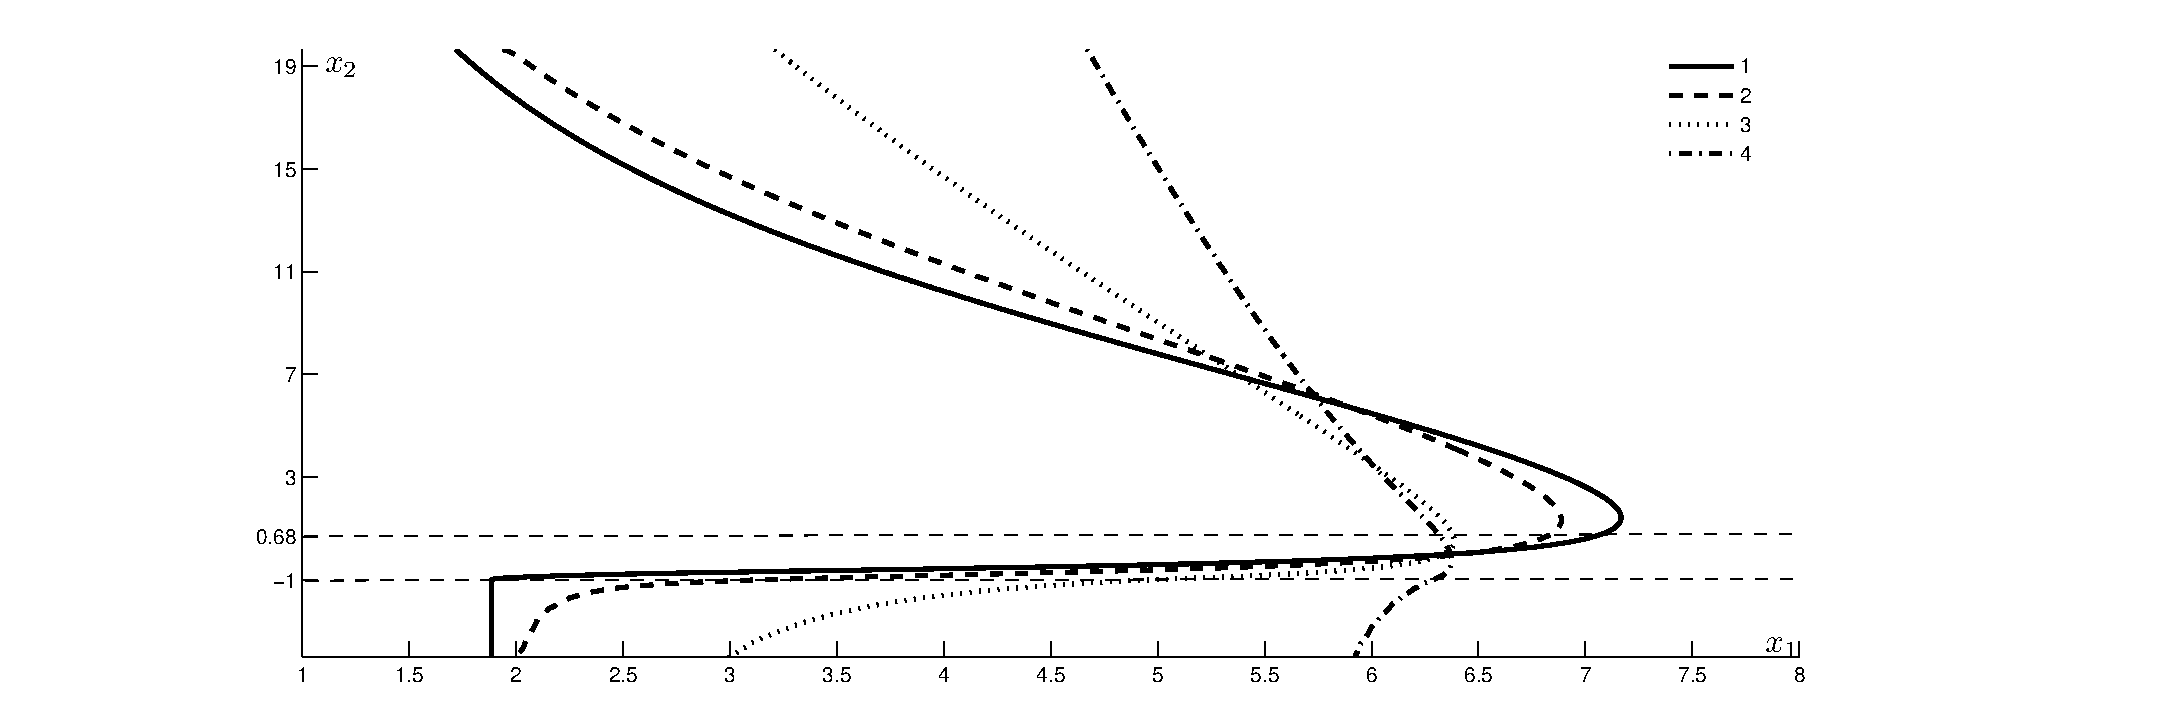
\includegraphics[width=1.1\textwidth]{C_1_f}
         \caption{График линии переключения $x^*(x_2)$ оптимальной стратегии $c^*$ выплаты дивидендов}
          \label{fig:1.2}
\end{figure}

График линии переключения $x^*(x_2)$ представлен на рис.\,\ref{fig:1.2}. При $\mu_2(x_2)<0$ (т.е. $x_2<-1$) в одномерной задаче линия переключения не зависит от $x_2$. Это объясняется тем что при этом $\theta^*=0$, и коэффициенты уравнения  (\ref{eq:1.2.1A}) не зависят от $x_2$. Далее, все графики линий переключения имеют точку глобального максимума.
Это можно объяснить спецификой модели Блэка-Шоулза, а именно тем, что
$$ \lim_{t\to\infty} S_t=\left\{\begin{matrix}
  0 &\text{при}& \mu_2(x_2)<\sigma_2^2(x_2)/2\\
  +\infty&\text{при}& \mu_2(x_2)>\sigma_2^2(x_2)/2
 \end{matrix}\right.
$$
при фиксированном $x_2$. Если значения параметра $x_2$ превосходят корень уравнения $\mu_2(x_2)=\sigma_2^2(x_2)/2$ (точка $\widehat x_2=0.68$ на рис.\,\ref{fig:1.2} ), то рисковый актив становится <<слишком хорошим>>. При дальнейшем увеличении $x_2$ это позволяет постепенно снижать уровень капитала фирмы, начиная с которого производится выплата дивидендов. Можно ожидать, что $x^*(x_2)\to 0$ при $x_2 \to +\infty$. Отметим также, что двумерный эффект выражается в том, что при увеличении $k_2$ график $x^*(x_2)$ становится более пологим и приближается к прямой $x_1=x^*(0)$.

Теперь рассмотрим поведение $\theta^*$ --- оптимального объема капитала, инвестируемого в рисковый актив.
\begin{figure}[h]
        \centering
          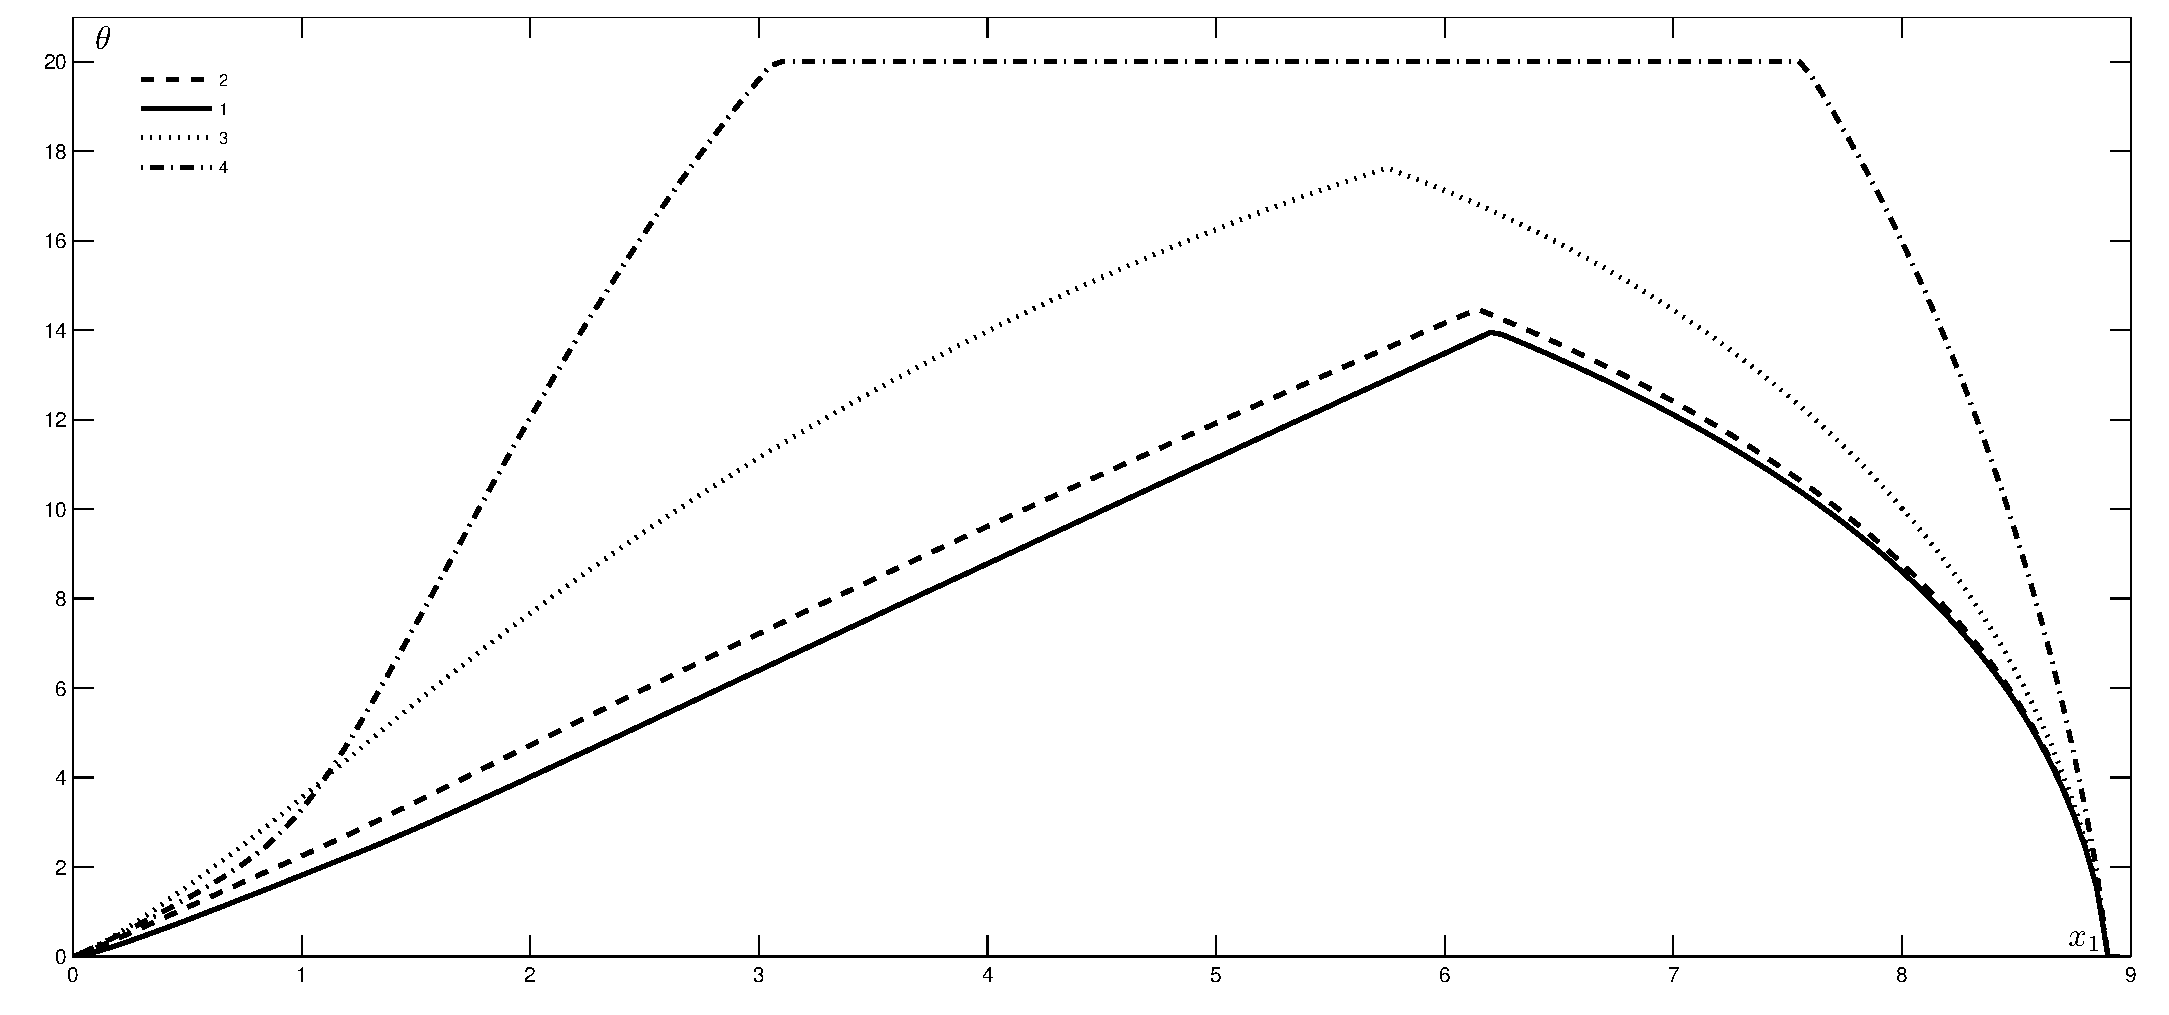
\includegraphics[width=0.8\textwidth]{th_1}
          %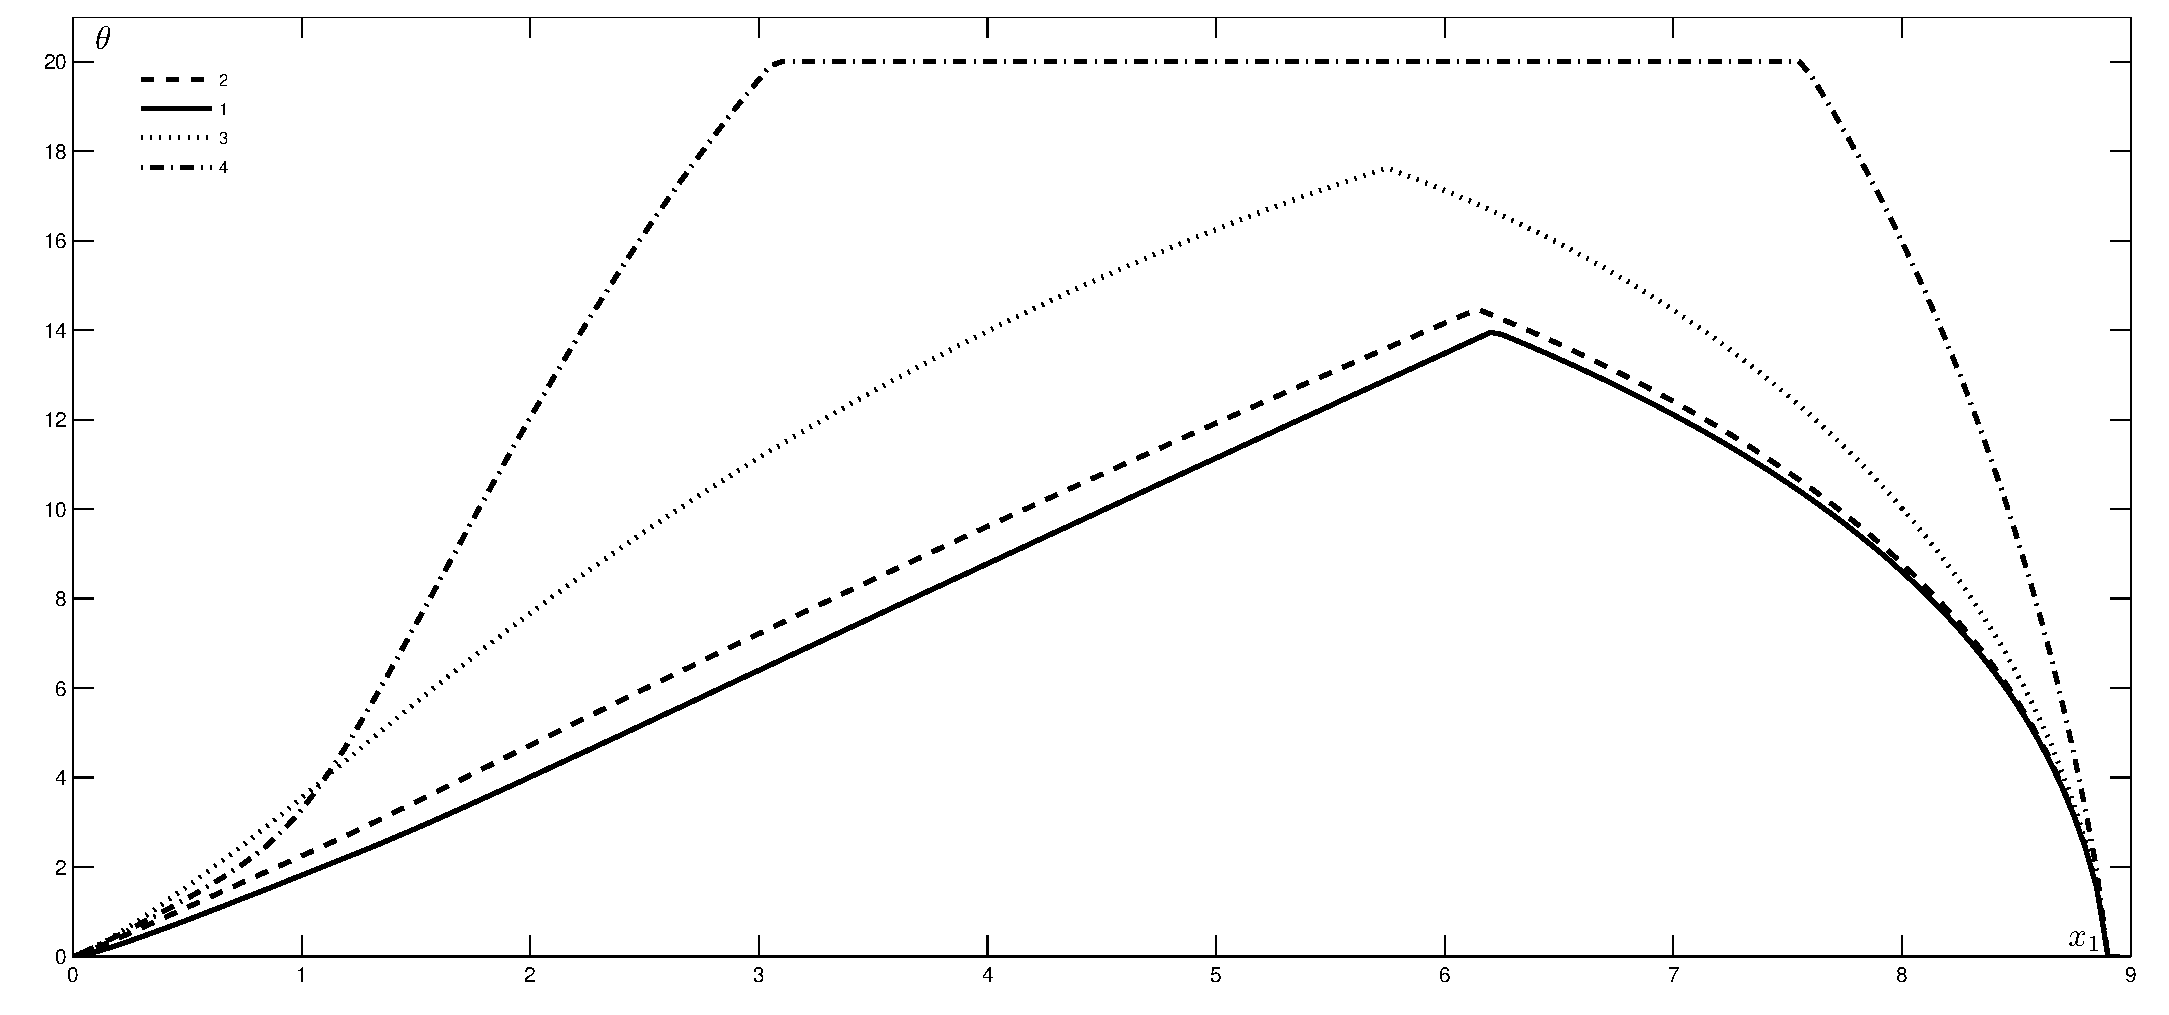
\includegraphics[trim=1mm 2mm 3mm 4mm]{th_1}
         \caption{Графики сечений $\theta^*(\cdot,x_2)$ при $x_2=5$.}
          \label{fig:1.3}
\end{figure}
Численные результаты показывают, что для любого фиксированного значения $x_2$ с $\mu_2(x_2)>0$ функция $x_1\mapsto \theta^*(x_1,x_2)$ возрастает на интервале $[0,x^*(x_2)]$ и убывает при $x_1>x^*(x_2)$ (в случае $k_2=10$  на рис.\,\ref{fig:1.3} имеется плоский участок графика, что соответствует достижению $\theta^*$ максимально допустимого значения $\overline\theta$). Интересный эффект падения $\theta^*$ при $x_1>x^*(x_2)$ по-видимому не описан в литературе применительно к данной задаче. Его можно объяснить тем, что увеличение капитала $V$ в данной области не приводит к увеличению скорости выплаты дивидендов. Как следствие меняется стратегия: увеличение капитала перестает быть приоритетом, что приводит к снижению волатильности оптимального портфеля.

%Отметим что по сравнению с классической задачей Мертона, где количество капитала, инвестируемого в рисковый актив, растет пропорционально общему капиталу, данное поведение $\theta$ выглядит необычно. Падение $\theta$ при $x>x^*(y)$ можно объяснить тем, что увеличение капитала компании в данной области не приводит к увеличению скорости выплаты дивидендов. Как следствие меняется стратегия: увеличение капитала перестает быть приоритетом, что приводит к снижению волатильности оптимального портфеля.
%Отметим, что, как показывают расчеты, в области $y: \mu2(y) \le 0$ имеет место очевидное равенство $\theta=0$.

Представляет интерес также поведение функции $x_2\mapsto\theta^*(x_1,x_2)$.
\begin{figure}[h!]
        \centering
          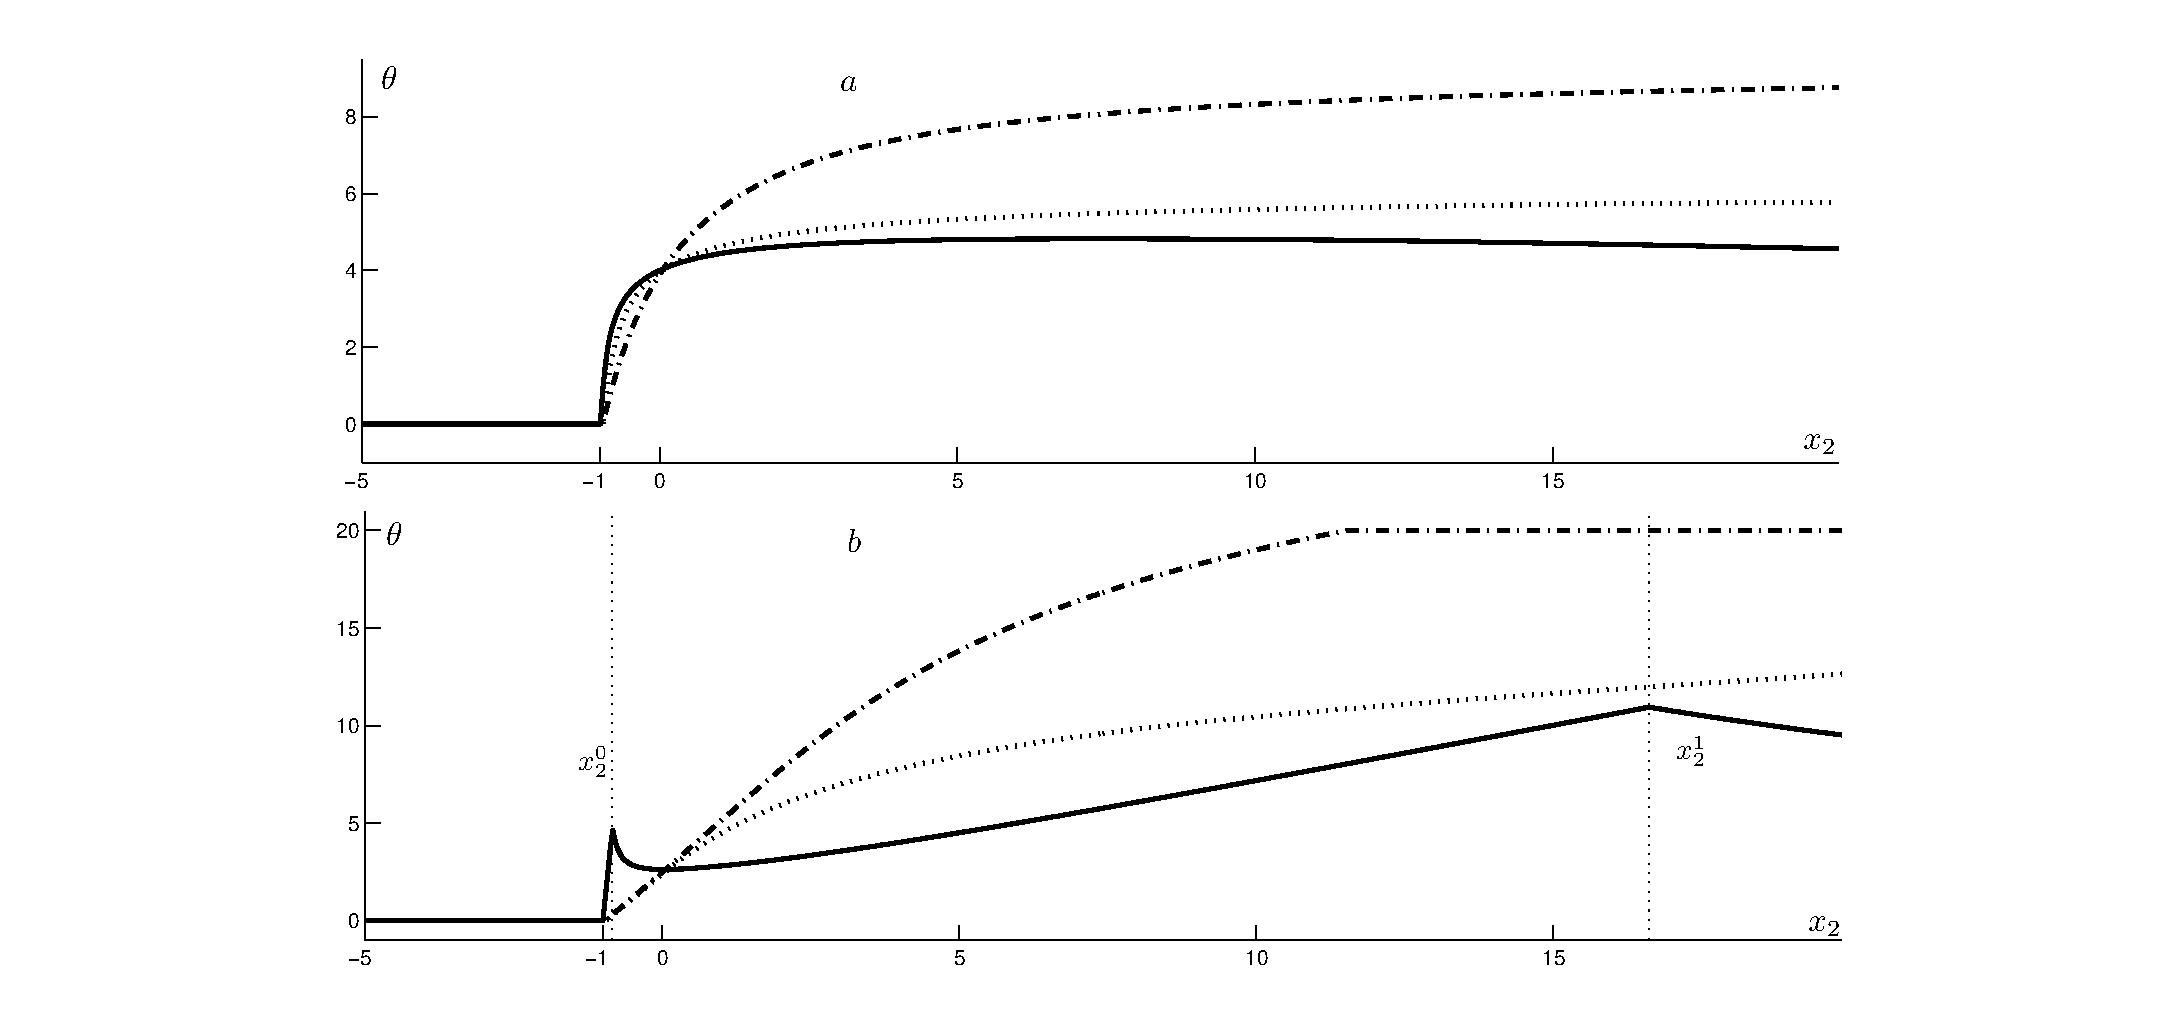
\includegraphics[width=0.9\textwidth]{th_3}
         \caption{Графики сечений $\theta^*(x_1,\cdot)$ при (a) $x_1=8.65$, (b) $x_1=5$.}
          \label{fig:1.4}
\end{figure}
Типичные графики представлены на рисунке \ref{fig:1.4}. С качественной точки зрения свойства данной функции, определяются числом пересечений прямой, проходящей через точку $x_1$ и параллельной оси $x_2$, с границей области выплаты дивидендов. Особенно ярко данный эффект проявляется в одномерной модели с параметром $x_2$.  На рисунке \ref{fig:1.4}(а) представлен случай, когда кривая $x_1=x^*(x_2)$, соответствующая одномерной модели, не пересекается с прямой $x_1=8.65$, а на рисунке \ref{fig:1.4}(б) --- случай, когда имеются два корня $x_2^0$, $x_2^1$  уравнения $x^*(x_2)=5$.

Двумерные эффекты состоят в сглаживании графиков и увеличении значений функции $\theta^*$ с ростом $k_2$. При этом монотонность функции $\theta^*(x_1,\cdot)$ в области невыплаты дивидендов можно объяснить сглаживанием, а увеличение $\theta^*$ с ростом $k_2$ --- желанием компании максимально использовать <<хорошие>> условия на рынке, пока они не вернулись к обычному уровню.
\begin{figure}[h!]
        \centering
          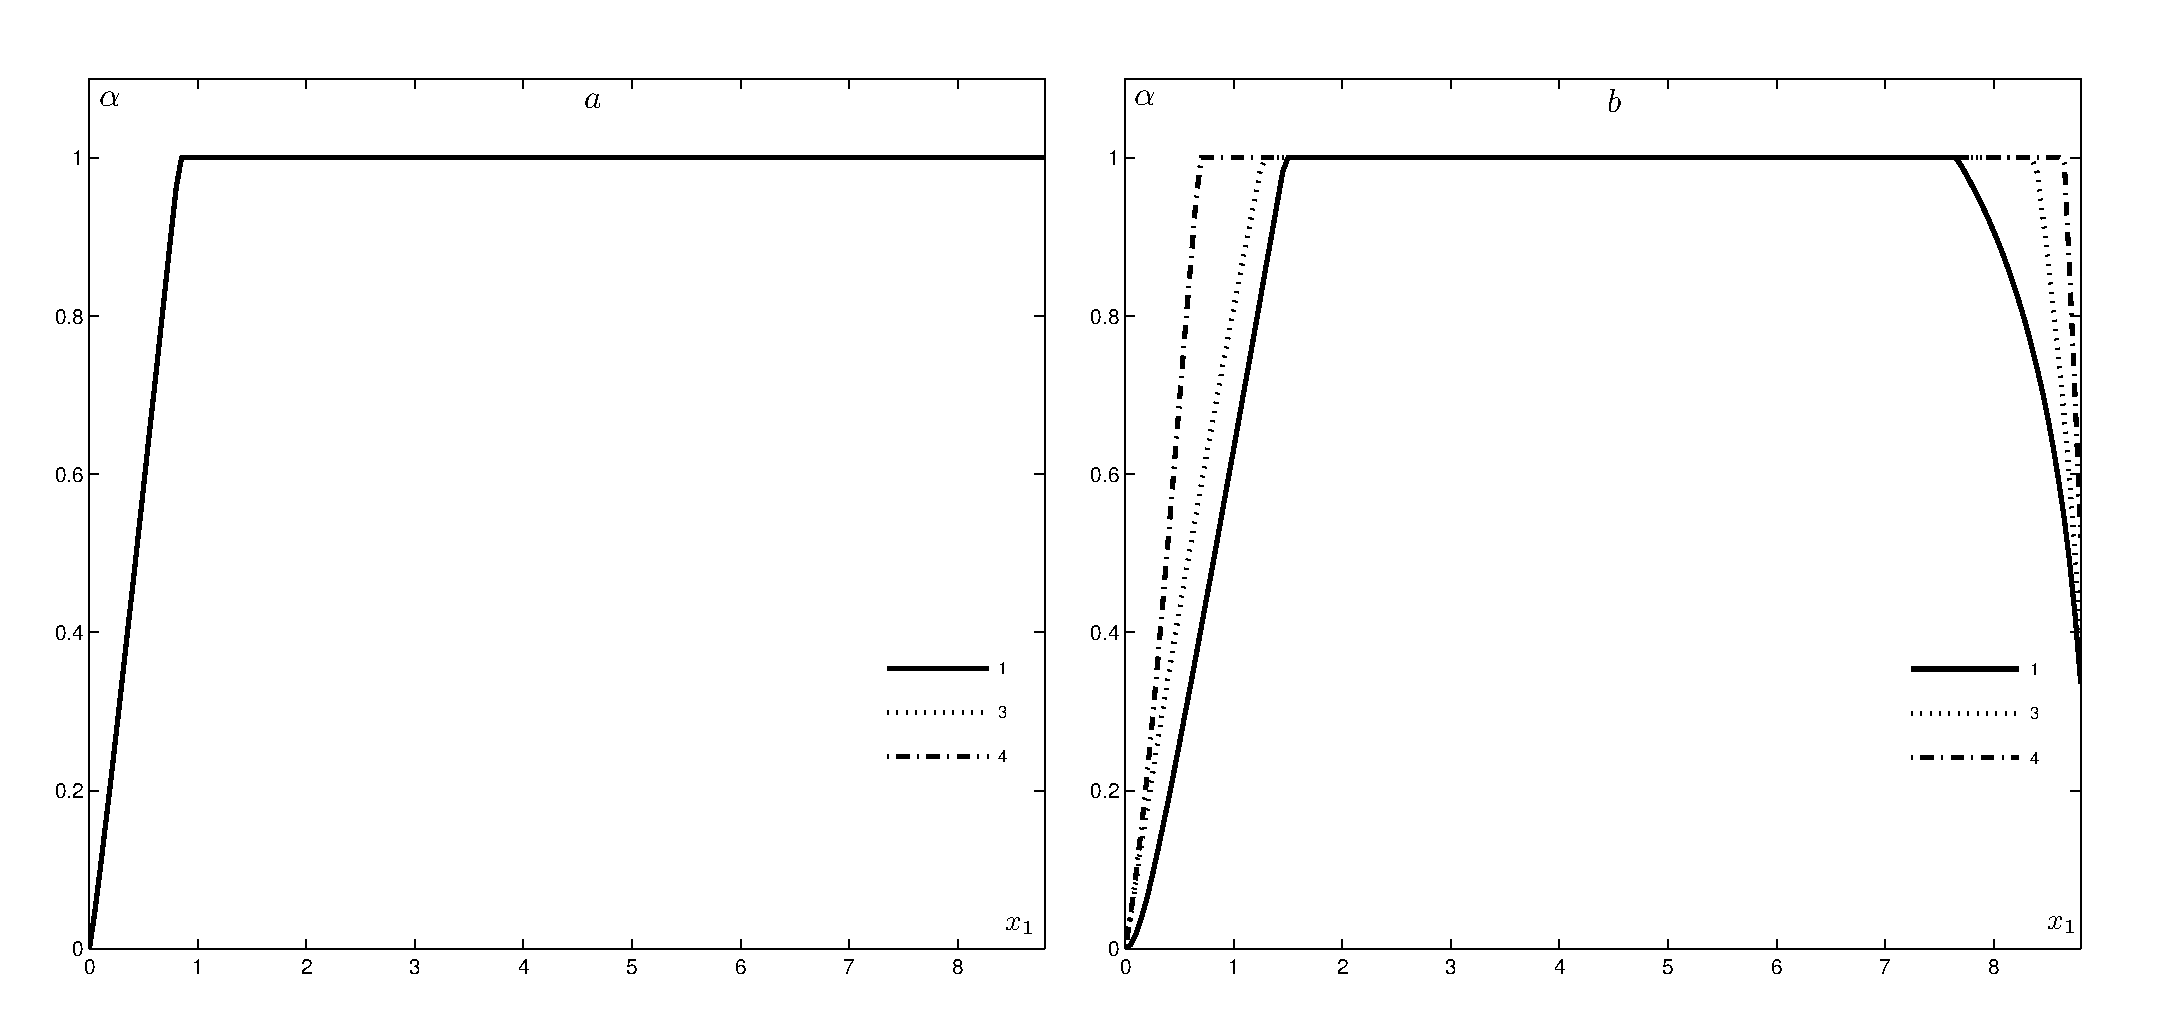
\includegraphics[width=0.85\textwidth]{alf_1}
         \caption{Графики сечений $\alpha^*(\cdot,x_2)$ при (a) $x_2=-4.17$, (b) $x_2=18.92$.}
          \label{fig:1.5}
\end{figure}

Рассмотрим, наконец, оптимальный уровень перестрахования. На представленных на рис.\,\ref{fig:1.5} графиках выделено два случая. При $\mu_2(x_2) \le 0$ поведение $\alpha^*$ соответствует описанному в работе \cite{AsmHojTak00}: имеется точка $\hat x \in (0,x^*)$ такая, что $\alpha^*$ возрастает по $x_1$ на интервале $(0,\hat x)$ и $\alpha^*=1$ при $x_1 \ge \hat x$. На рис.\,\ref{fig:1.5}(a) представлен одномерный случай. В двумерном случае, для любого значения параметра $k_2$ график остается тем же. Причина состоит в том, что в области $\mu_2(x_2) \le 0$ не задействован инвестиционный портфель: $\theta^*=0$.

При $\mu_2(x_2)>0$ возникает эффект падения $\alpha^*$ при больших значениях $x_1$: рис.\,\ref{fig:1.5}(b).
\begin{figure}[h!]
        \centering
          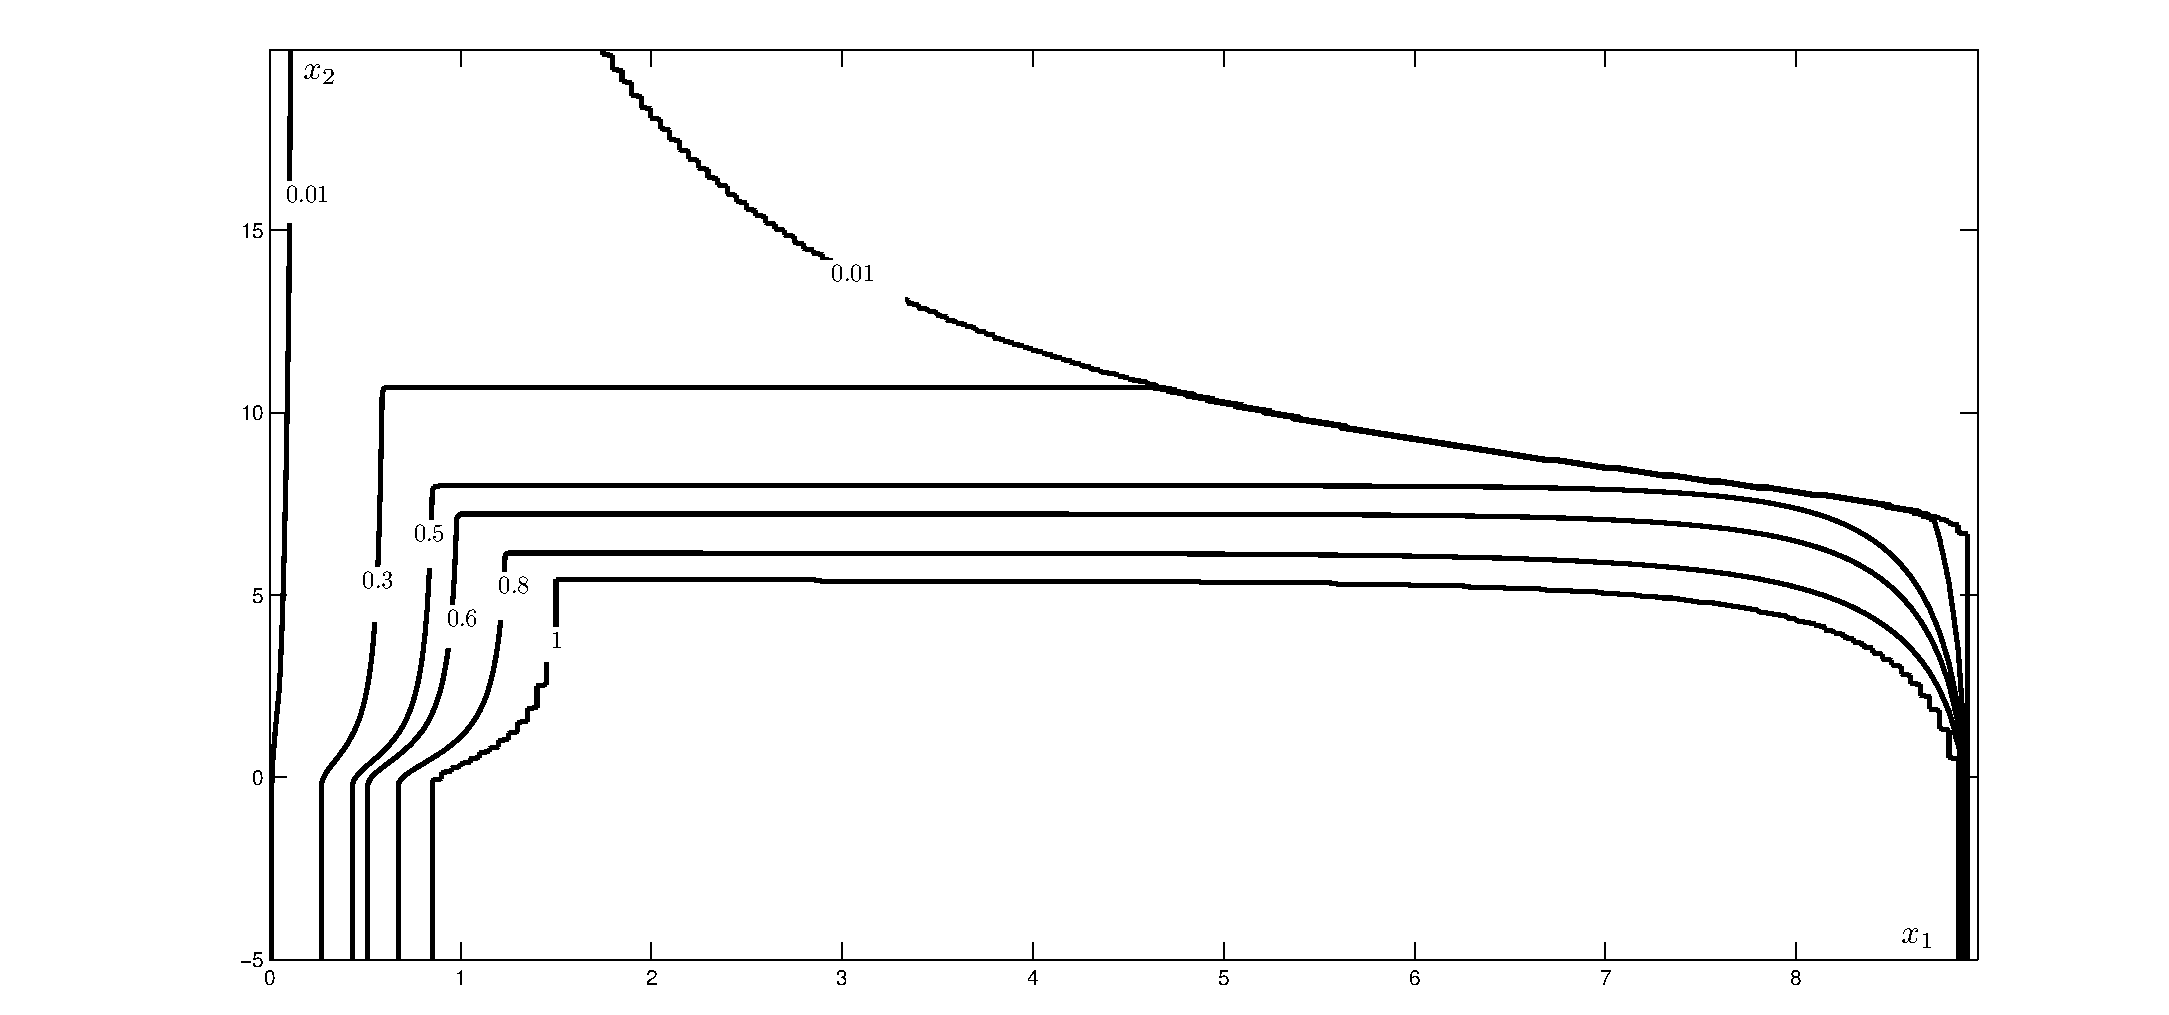
\includegraphics[width=0.85\textwidth]{alf_2}
         \caption{Линии уровня $\alpha^*$, в случае одномерной модели с параметром $x_2$.}
          \label{fig:1.6}
\end{figure}
То, что этот эффект реален и не связан с искажениями, которые вносятся искусственным граничным условием $v(\overline x_1, x_2)=0$,
подтверждается линиями уровня $\alpha^*$, соответствующими одномерной задаче с параметром $x_2$: см. рис.\,\ref{fig:1.6}. Заметим, что функция $x_2\mapsto\alpha^*(x_1,x_2)$ является убывающей и $\max_{x_1}{\alpha^*}(x_1,x_2)<1$ при больших значениях $x_2$.
Убывание $\alpha^*$ по $x_2$, означает, что при увеличении $x_2$ страховая компания постепенно превращается в инвестиционную. В двумерном случае (который не представлен на рисунках) ситуация сложнее. В частности, монотонное убывание функции $\alpha^*$ по $x_2$ наблюдается лишь при достаточно больших значениях $x_1$.
%\newpage
%============================================================================================================================

%\subsection{Ненумерованные многострочные формулы} \label{subsect:1.4.1}
%\newpage
%============================================================================================================================

\clearpage 